\cleardoublepage

\chapter{Modelización estructural}
\label{makereference5}

Una vez obtenidos tanto los datos de las señales de la infraestructura operacional y la información del entorno del mercado, es necesario realizar un modelado estructural del entrono a optimizar para, tomadas las entradas, determinar la posición del mercado óptima de las baterías.

Exactamente, el objetivo principal de la etapa de optimización del sistema es responder a las cuestiones de cuándo y de qué fuente ciclar energía y cuánta energía ciclar, buscando siempre los mayores ingresos.

Para ello, se ha elegido Pyomo como herramienta de modelización matemática en el área de investigación operacional. Pyomo es una librería de Python para formular, solucionar y analizar problemas de optimización, como el propio.

Se hace uso de una formulación de \gls{milp} para poder tener en cuenta condiciones más allá de la más simple \gls{lp}. Se ha explorado el uso de indicadores o restricciones avanzadas, como los \textit{special order sets}, los cuales han sido descartados en última instancia debido a problemas de rendimiento. Esto significa que la modelización es puramente de enteros mixtos compatible con cualquier solucionador que soporte variables binarias.

De esta forma, se detallan los parámetros de decisión en la sección~\ref{makereference5.1}, que articulan el problema de optimización, abarcando desde la definición temporal de los periodos del mercado y las variables de operación de los flujos energéticos, hasta las limitaciones impuestas por el comportamiento físico de la batería y las guías estratégicas de las indicaciones de mercado. Se procede a formular las restricciones operacionales que aseguran la viabilidad técnica de la solución en la sección~\ref{makereference5.2}, se habla de la optimización dual de la instalación al completo de la generación energética en la sección~\ref{makereference5.3}, se establece el criterio de desempeño que define la función objetivo a optimizar en la parte~\ref{makereference5.4} y, finalmente, se consideran los requisitos de la resolución numérica para cumplir con la precisión exigida por el operador del mercado en la sección~\ref{makereference5.5}.

\section{Parámetros de decisión}
\label{makereference5.1}

Todo modelado estructural debe contar inicialmente con un conjunto de parámetros de decisión que determinen los valores con los que trabaja el modelo. Más adelante, dichos parámetros son usados para definir las restricciones que el control de la batería debe cumplir.

\subsection{Periodos del mercado}
\label{makereference5.1.1}

El mercado eléctrico peninsular opera en etapas discreta temporales con una granularidad establecida. Los mercados spot, de los que se encarga el sistema en la actualidad, disponen de una granularidad horaria para el mercado diario\footnote{La granularidad del mercado diario se encuentra en proceso de actualización a cuartohoraria} y cuartohoraria para los mercados intradiarios y el mercado intradiario continuo. En el resto de mercados de Europa, como Nord Pool, la granularidad de los mercados spot es similar, existiendo también granularidades incluso de 30 minutos.

La variabilidad de la granularidad exige representar el mercado en múltiples periodos categóricos de tamaño proporcional. De esta forma, el sistema representa el mercado mismo mediante la ecuación~\ref{eq:set-mercado}.

\begin{samepage}

  \begin{equation}
    \label{eq:set-mercado}
    T = \{t_{0} + k \cdot \Delta t \mid k \in \mathbb{N}_{0}, t_{0} + k \cdot \Delta t \leq H\}
  \end{equation}

  donde

  \begin{itemize}

    \item \( T \) es el conjunto de todos los períodos de tiempo discretos.

    \item \( t_0 \) es el tiempo inicial del conjunto.

    \item \( k \) es el contador de pasos, que es un número natural (incluido el cero), \( k \in \{ 0, 1, 2, 3, \dots \} \).

    \item \( \Delta t \) es la granularidad o el tamaño del paso de tiempo entre un período y el siguiente.

    \item \( H \) es el horizonte de optimización, que marca el límite superior o el tiempo final de la serie temporal.

  \end{itemize}

\end{samepage}

Es necesario tener en cuenta los usos horarios a la hora de calcular el tamaño del mercado, ya que los mercados siempre y en todo momento hacen uso del uso horario local, a diferencia de UTC. Esto significa que en los día de cambio de hora, los mercados del día tendrán más o menos periodos y el mercado intradiario continuo tendrá más o menos sesiones, dependiendo de si se añaden o restan horas. El operador del mercado lo detalla en la tabla~\ref{tab:cambio-hora}.

\begin{table}[ht]
  \centering
  \begin{tabular}[c]{|l|l|l|}
    \hline
    Código & Descripción & Tipo de producción\\
    \hline
    \hline
  \end{tabular}
  \caption[Ajustes del mercado en cambios de hora.]{Ajustes del mercado en cambios de hora.}
  \label{tab:cambio-hora}
\end{table}

La representación del mercado durante la optimización realmente incluye multiples posibles mercados futuros más allá del más proximo, es decir, el sistema tiene en cuenta un horizonte de optimización de varios mercados y, por lo tanto, varios periodos a lo largo de múltiples días de mercado. La razón de lo cual reside en facilitar la mayor información posible: si un día de mercado no cumple con las condiciones de actuación mientras que otro día de mercado las dobla, es posible no arbitrar uno de los días y ofertar el doble el otro, en vez de perder la oportunidad, representado en la figura~\ref{fig:horizonte-de-optimizacióno}.

\begin{figure}
  \centering
  % \includegraphics[width=0.5\linewidth]{figures/horizonte-de-optimizacióno.jpg}
  \caption[Representación del horizonte de optimización.]{Representación del horizonte de optimización.}
  \label{fig:horizonte-de-optimizacióno}
\end{figure}

\subsection{Flujos energéticos}
\label{makereference5.1.2}

El mercado, precisamente, es usado para indexar los flujos energéticos explicados en la sección~\ref{makereference3.1} de infraestructura operacional. Estos flujos energéticos representan la operación y, por lo tanto, salida de la optimización. Responden a las tres preguntas planteadas anteriormente.

La configuración topológica más simple, la configuración topológica aislada, tan solo dispone de dos: el flujo de importación de la red al sistema de almacenamiento de energía en baterías y exportación del sistema de almacenamiento de energía en baterías a la red. La configuración topológica añade uno más, la importación de la generación al sistema de almacenamiento de energía en baterías.

Aún así, ellos solos no bastan para controlar la batería correctamente. Para ello, conviene más observar estos flujos energéticos no como flujos energéticos mismos, sino como interfaces de compra y venta, como las unidades físicas explicadas en el apartado~\ref{makereference4}. Realmente, el sistema se encarga de arbitrar en el mercado, por lo que debe operar no solo en la capa de abstracción de flujos energéticos físicos, sino además en la de los movimientos del mercado.

Todo esto es para subrayar que los flujos energéticos, desde la perspectiva del mercado, no están limitados a únicamente a la dirección de compra para la carga y venta para la descarga. Una unidad física correspondiente a la importación de energía es capaz de venderla también, solo que esa energía vendida no puede provenir de la instalación perteneciente a la unidad física, ya que el flujo energético fisco limita la venta.

Por ejemplo, como se realizan varias sesiones de mercado en un mismo día, puede que el sistema haya prometido vender una cantidad de energía en un periodo de la tarde en el mercado diario. Lamentablemente, una hora antes de tener que exportar toda esa energía casada (en la última sesión del mercado intradiario continuo antes del \textit{delivery}), resulta que las nuevas previsiones meteorológicas indica que, debido a una nube repentina, los paneles fotovoltaicos no van a ser capaces de generar la suficiente energía como para cargar la batería y exportar su energía. Esto genera un desvío en la posición de la batería: no va a ser capaz de otorgar toda la energía prometida y puede resultar penalizada. Por suerte, como se ha explicado, la solución al problema es recomprar la cantidad de energía que le falte al sistema a través de la interfaz de exportación. Como las recompras (y reventas, en el caso contrario) se realizan exclusivamente en el mismo periodo de su correspondiente posición opuesta por definición, la energía no necesita pasar por la interfaz que ha realizado la operación y la instalación puede exportar la energía tranquilamente y suplir la falta al mismo tiempo, sin tener que importan energía a la instalación.

Por lo tanto, los diferentes flujos energéticos son representados de la siguiente forma, correspondientes con los resultados principales de la optimización

...

\subsection{Comportamiento físico}
\label{makereference5.1.3}

Aunque los anteriores flujos energéticos sean dependientes de la configuración topológica, toda batería comparte unos comportamientos físicos intrinsecos. Al fin y al cabo, las baterías son sistemas de almacenamiento de energía que permiten ser cargadas para su posterior descarga, pero ¿cómo de rápido pueden ser cargadas y descargadas, cuánto, cuántas veces, etc.?

Precisamente, las señales configuradas propiamente en el sistema de información de planta detalladas en la sección~\ref{makereference3.2} permite conocer los parámetros operacionales de las batería. Con ellos, lo que es necesario es representarlos por el sistema para su optimización operativa.

...

\subsection{Indicaciones de mercado}
\label{makereference5.1.4}

Finalmente, los previos parámetros completan la modelización de la batería, en cambio, el sistema debe ser capaz de guiar la operación de la batería. Es decir, impedir situaciones posibles físicamente realizables por la batería pero que no interesan.

Para ello, el sistema define el ingreso obtenido y los ciclos realizados como los principales indicadores de rendimiento, por lo tanto, se expresan los siguientes parámetros que los controlan.

...

\section{Restricciones operacionales}
\label{makereference5.2}

Conociendo los parámetros con los que trabaja el apartado de optimización del sistema, es momento de definir las restricciones operacionales que establecen las relaciones entre ellos. Las ecuaciones mostradas se encuentran simplificadas para facilitar la comprensión aunque resulten más robustas en la realidad. No se muestran, por ejemplo, las restricciones de consignación manual tanto de la posición como el estado de carga, explicadas en el apartado~\ref{makereference6}.

Como algunas configuraciones topológicas no soportan todos los flujos energéticos, como la importación de la red en la híbrida con carga aislada de la red o la importación de la generación en la aislada, estas deben ser capaces de ser desactivadas a través de la simple formula~\ref{eq:desactivación-ufi}.

\begin{equation}
  \label{eq:desactivación-ufi}
\end{equation}

Con esto, los flujos energéticos netos están definidos como la suma del correspondiente flujo energético bruto y el casado, es decir, el flujo energético físico representado por el parámetro neto debe ser siempre no negativo, pero la interfaz de la unidad física lo puede ser cuando existan posiciones casadas en un periodo concreto. Esto es representado por la ecuación~\ref{eq:neto-bruto} y se realiza para cada uno de los flujos energéticos con unidades físicas arbitrados en el mercado, es decir, la importación de la red y la exportación a la red.

\begin{equation}
  \label{eq:neto-bruto}
\end{equation}

Con respecto a los parámetros del comportamiento físico, estos limitan la potencia tanto de carga como de descarga\footnote{Aunque la potencia de carga y descarga generalmente coincida en las instalaciones para las que se ha desplegado el sistema, es importante reconocer que pueden no ser iguales} mediante la ecuación~\ref{eq:capacidad-potencia-carga} de carga y la ecuación~\ref{eq:capacidad-potencia-descarga} de descarga. La señal de disponibilidad afecta linealmente a la capacidad de potencia, para una disponibilidad de la mitad, la potencia de la batería es la mitad misma de su capacidad nominal.

\begin{equation}
  \label{eq:capacidad-potencia-carga}
\end{equation}

\begin{equation}
  \label{eq:capacidad-potencia-descarga}
\end{equation}

Y junto a la potencia, la capacidad de almacenamiento la limita el correspondiente parámetro nominal de la batería en~\ref{eq:capacidad-almacenamiento}.

\begin{equation}
  \label{eq:capacidad-almacenamiento}
\end{equation}

Las eficiencias de carga y descarga también afectan al ciclado. Precisamente, es absolutamente necesario separar la carga por un lado y la descarga por otro ya que una de los indicadores de rendimiento es el número de ciclos. Como se indica oficialmente: "se completa un ciclo de carga cuando se ha usado (descargado) una cantidad equivalente al 100 \% de la capacidad de la batería, pero no necesariamente toda con una sola carga. Por ejemplo, podrías usar el 75 \% de la capacidad de la batería un día y luego recargarla completamente durante la noche. Si usas el 25 \% al día siguiente, habrás descargado el 100 \% en total, y los dos días sumarán un ciclo de carga."

Esto significa que si la carga y la descarga no se separase, el número de ciclos sería contado incorrectamente ya que podrían realizarse ciclos que dejasen la batería en el mismo estado, y seguir siendo ciclos perfectamente válidos. De esta forma, las ecuaciones de las eficiencias detallan la carga proveniente tanto de la importación de la red y de la importación de la generación en~\ref{eq:eficiencia-carga} y la descarga en~\ref{eq:eficiencia-descarga}.

\begin{equation}
  \label{eq:eficiencia-carga}
\end{equation}

\begin{equation}
  \label{eq:eficiencia-descarga}
\end{equation}

Aún así, separar la carga y la descarga introduce uno de los mayores problemas del sistema, la carga y descarga simultanea. La defensa ante esta situación, invalida físicamente debido al funcionamiento de la conexión interna de las baterías, es realizada para la consignación en la sección~\ref{makereference6.1.1}. Durante la optimización, en cambio, se tiene en cuenta usando la programación de enteros mixtos previamente mencionada y sus pertinentes variables binarias en la formulación~\ref{eq:carga-descarga-simultánea}.

\begin{equation}
  \label{eq:carga-descarga-simultánea}
\end{equation}

Un aspecto a tener en cuenta es que la formulación puede realizarse usando \textit{special order sets} para evitar el uso de variables Big M, como se indica en la ecuación~\ref{eq:carga-descarga-simultánea-sos}. Si las variables de carga y descarga (y el resto más adelante) no estuvieran limitadas físicamente (Big M arbitrariamente alto), esto podría afectar negativamente al rendimiento del sistema, pero como sí lo están, no existen problemas de estabilidad numérica.

\begin{equation}
  \label{eq:carga-descarga-simultánea-sos}
\end{equation}

El indicador de mercado de ciclos máximos limita simplemente los ciclos mediante la ecuación~\ref{eq:limite-ciclos}. Para no introducir relaciones no lineales y afectar negativamente al rendimiento del sistema, el indicador de mercado de ciclos máximos proviene de la verdadera opción de configuración expuesta a los agentes de mercado y operadores de telecontrol en forma de ciclos máximos por día y multiplico directamente por el número de días del horizonte de optimización \( ... \). Aunque esto conlleva que los ciclos puedan repartirse a lo largo del horizonte de optimización, a diferencia de una solución no lineal, no es ningún problema, verdaderamente.

\begin{equation}
  \label{eq:limite-ciclos}
\end{equation}

El estado de carga lo limitan las señales de la batería en la ecuación~\ref{eq:limite-soc}. Generalmente, se suele dejar una cantidad de energía disponible continuamente para evitar imprevistos.

Precisamente, un efecto secundaria inmensamente beneficioso de las limitaciones de la señal del estado de carga es la posibilidad de la participación de las baterías en los mercados de disponibilidad\footnote{El sistema no soporta los mercados de disponibilidad en su estado actual, aunque sí que permite manejarlos externamente}. Como en ningún momento se llega ni al máximo ni al mínimo de la capacidad de la batería, esta puede ofertar por lo menos el rango del estado de carga a subir o bajar y generar beneficios pasivos sin afectar de ninguna forma a la operación principal en los mercados spot.

\begin{equation}
  \label{eq:limite-soc}
\end{equation}

Continuando con el estado de carga, es necesario conocer por lo menos el estado de carga inicial de donde se parte, ecuación~\ref{eq:soc-inicial}, y también determinar asignar el estado de carga final, ecuación~\ref{eq:soc-final}, para ejecutar grupos de ciclado consistentes en donde el estado de carga de la batería no termine en un valor indeterminado.

\begin{equation}
  \label{eq:soc-inicial}
\end{equation}

\begin{equation}
  \label{eq:soc-final}
\end{equation}

De esta forma, se define la ecuación del estado de carga~\ref{eq:soc}, teniendo en cuenta la energía cargada y descargada.

\begin{equation}
  \label{eq:soc}
\end{equation}

Ademas, la modelización también debe tener en cuenta las limitaciones de programa obtenidas en la sección~\ref{makereference4.2.1}. Estas limitaciones impiden la exportación de energía de cada uno de los activos energéticos individualmente.

...

Esta nueva restricción, en cambio, introduce nuevas oportunidades de arbitraje ya que las limitaciones no son de la instalación al completo (también), sino individuales según el activo energético. Esto significa que puede que la generación se vea limitada (el funcionamiento de la misma es explicado en la sección~\ref{makereference5.3}) pero no la exportación de la batería. Ante dicha situación, la batería es capaz de cargarse sin ningún coste.

Para tener mejorar el rendimiento y tener en cuenta esos escenario, se introducen nuevas restricciones en forma de la ecuación~\ref{eq:curtailed-import}, que controla la importación de energía excedente, y la ecuación~\ref{eq:uncurtailed-import}, que controla la importación de energía no excedente. De hecho, el termino usado para referirse a la energía excedente se conoce como \textit{curtailment}.

\begin{equation}
  \label{eq:curtailed-import}
\end{equation}

\begin{equation}
  \label{eq:uncurtailed-import}
\end{equation}

Estas nuevas restricciones, lamentablemente, introducen otro nuevo conflicto. ¿Cómo se decide si cargar de la energía excedente o de la no excedente? Entendiblemente, siempre es necesario priorizar la carga de la energía excedente, por lo que se añade otra indicación de enteros mixtos a la formulación, ecuación~\ref{eq:indicador-curtailment}. De la mismo forma que el Big M anterior, la importación tanto excedente como no excedente cuenta con un límite superior en forma de la cantidad de energía disponible, por lo que no existen problemas de estabilidad numérica directos.

\begin{equation}
  \label{eq:indicador-curtailment}
\end{equation}

Para terminar con lo relacionado con los sistemas de almacenamiento de energía en baterías mismos, por el momento solo se ha tenido en cuenta una configuración topológica del estilo de la aislada e híbrida flexible, ya que, según se ha descrito hasta ahora, el sistema puede importar energía de la red o de la generación libremente (bajo el resto de restricciones).

En cambio, no todas las configuraciones topológicas operan de la siguiente manera. Precisamente, la híbrida con carga aislada de la red muestra un comportamiento de \textit{clipping}, en donde existe una cantidad de energía excedente de donde la batería solo puede cargar.

Representado en la figura~\ref{fig:clipping}, se puede entender como una persona que dispone de un salario fijo (generación). Cada mes debe pagar una cantidad de su salario para el alquiler (\textit{threshold} de carga). Del dinero sobrante, ahorra (carga) una porcentaje (coeficiente de \textit{clipping}), mientras que gasta el resto como le apetezca (exportación de generación).

\begin{figure}
  \centering
  % 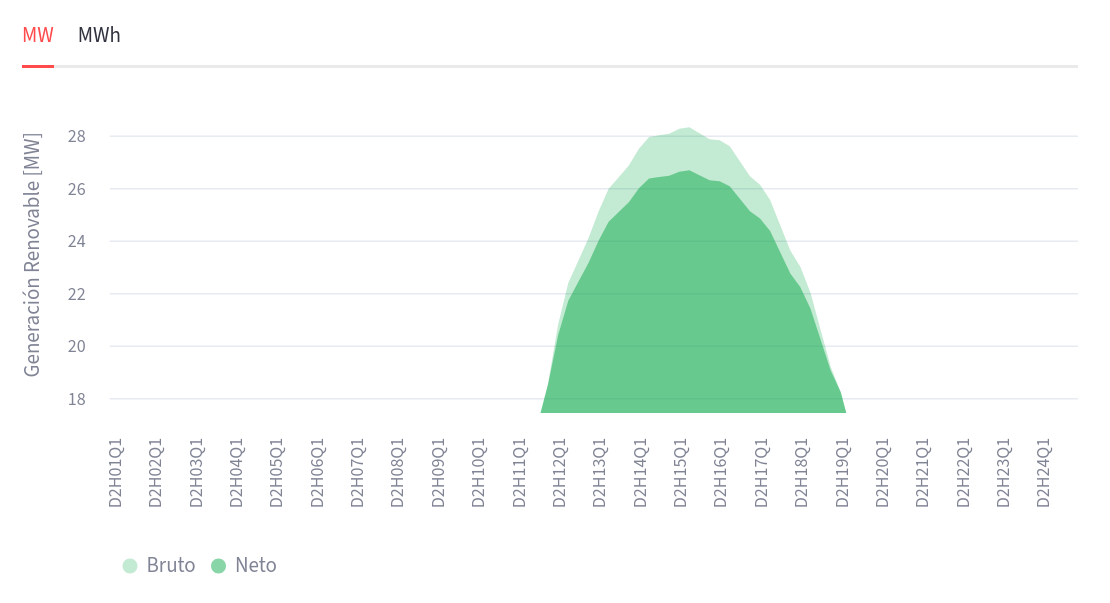
\includegraphics[width=0.5\linewidth]{figures/clipping.jpg}
  \caption[Clipping de configuración topológica híbrida.]{Clipping de la configuración topológica híbrida con carga aislada de la red.}
  \label{fig:clipping}
\end{figure}

El sistema lo representa mediante la ecuación~\ref{eq:clipping}.

\begin{equation}
  \label{eq:clipping}
\end{equation}

La última configuración topológica a tener en cuenta se trata de la híbrida con prioridad de carga de generación. Esto significa que se debe agotar completamente el recurso de generación antes de poder cargar de la red, aunque cargar de la red otorgue mayores beneficios, como es el caso de los precios de mercado negativos.

Dicha prioridad es definida de forma simular a previas restricciones de indicación Big M con enteros mixtos en la ecuación~\ref{eq:prioridad-híbrida}.

\begin{equation}
  \label{eq:prioridad-híbrida}
\end{equation}

Como se puede observar, el sistema es completamente genérico e incorpora comportamientos, a diferencia de definir entidades separadas para cada configuración. Es decir, el sistema usado es exactamente el mismo para cualquier configuración.

\section{Generación energética}
\label{makereference5.3}

Aunque, la modelización anterior cubra el comportamiento de los sistemas de almacenamiento de energía en baterías al completo, al sistema le surge un pequeño problema, ¿cómo decide cuándo cargar de la red o de la generación?

Las restricciones previas tan solo dibujan un marco general pero no tienen en cuenta que la energía importada de la generación es energía que la instalación, a través de la interfaz de exportación de la generación, no es capaz de vender, la carga de la batería lo impide.

Por lo tanto, es necesario tener en cuenta la generación junto con la batería y realizar una optimización de los flujos energéticos de la instalación al completo, incluida la generación. Si añadimos la generación al criterio de desempeño de la sección~\ref{makereference5.4}, la batería no podrá "robar" energía a la generación ya que debe existir una armonía conjunta en busca de la maximización del ingreso.

Precisamente y como se ha afirmado anteriormente, uno de los propósitos principales del sistema es su uso avanzado en instalaciones híbridas, como se puede observar.

...

\section{Criterio de desempeño}
\label{makereference5.4}

Como se ha mencionado en múltiples ocasiones, el criterio de desempeño del sistema parece ser el beneficio obtenido, es decir, el sistema busca maximizar los ingresos, en cambio, esto no es del todo cierto.

En el beneficio toma parte cada flujo de energía. Importantemente, como el sistema asume que las recompras y reventas se realizan al mismo precio que la posible compra y venta, tan solo se tienen en cuenta los flujos energéticos netos, correspondientes a los flujos físicos, para las interfaces de mercado. Con ello, se le asigna un precio a cada uno de ellos, resultando en la ecuación~\ref{eq:beneficio}.

\begin{equation}
  \label{eq:beneficio}
\end{equation}

Si bien la maximización del beneficio es uno de los objetivos, el principal precisamente, el sistema debe tener en cuenta otros factores. De hecho, cuando se realiza la optimización, tener en cuenta el beneficio unicamente resulta, casi con total certeza, en un problema de optimización degenerado.

Los problemas de optimización degenerados son los que poseen múltiples soluciones para una misma formulación. El sistema, por el contrario, debe asegurar una optimización determinista (llamada estricta) para facilitar el control de las baterías, no se puede permitir que ante cualquier modificación en su configuración, por muy minúsculo que sea, la posición óptica cambie drásticamente y genere desvíos. La diferencia se observa en la figura~\ref{fig:degenerada-vs-estricta}.

\begin{figure}
  \centering
  % \includegraphics[width=0.5\linewidth]{figures/degenerada-vs-estricta.jpg}
  \caption[Comparación entre una posición degenerada y estricta.]{Comparación entre una posición degenerada y su contraparte estricta.}
  \label{fig:degenerada-vs-estricta}
\end{figure}

Para solucionar este problema, se tiene en cuenta que las predicciones de precio de mercado y las predicciones meteorológicas, es decir, la información extraída en el apartado~\ref{makereference4} del entorno de mercado, es más precisa cuanto más cercana en el tiempo sea. En otras palabras, las previsiones para el día de mañana resultan más fiables que las de dentro de 5 días.

Dentro de la formulación, esta preferencia de las posiciones más cercanas en el tiempo se representa con una función de decrecimiento o \textit{decay function} exponencial, ecuación~\ref{eq:exponential-decay}. Dispone de un ratio de decrecimiento configurable dependiente del horizonte de optimización, cuanto mayor sea menor valor tendrá el ratio de decrecimiento, para evitar conflictos en donde peor posición más cercana en el tiempo sea elegido ante una mejor más lejana.

\begin{equation}
  \label{eq:exponential-decay}
\end{equation}

De esta forma, tras realizar el llamado test de factibilidad básica e identificar las variables básicas\footnote{Las variables básicas son las que marcan los puntos extremos de las soluciones, pero no tienen por que encontrarse en su límite, lo cual resultó ser fuente de confusión en el análisis de factibilidad} y sus propiedades, se determina la estrictez de la formulación.

\section{Optimización lexicográfica}
\label{makereference5.4.1}

Aunque el uso de una función de decrecimiento incorpore distinga correctamente las soluciones de forma determinista, técnicamente es posible, dependiendo de los parámetros de configuración, que la solución obtenida por el solucionador sea la óptima según el criterio de desempeño definido, pero no la que el sistema busca. Esto sucede debido a que parámetros de decisión incorrectamente seleccionados pueden priorizar una posición que mejore el objetivo de la preferencia temporal y no el del beneficio.

La metodología anterior de juntar los dos objetivos se conoce como optimización multiobjetivo ponderada, donde el coeficiente de ponderación es el calculado mediante la \textit{decay function} exponencial. Aún así, existe una técnica de optimización multiobjetivo más avanzada que evita conflictos entre ellos gracias a una metodología de priorización de objetivos, llamada optimización lexicográfica.

De esta forma, se desarrolla el algoritmo~\ref{alg:optimización-lexicográfica} de optimización lexicográfica multiobjetivo por encima del lenguaje de modelado abstracto para asegurar la priorización de los objetivos de la modelización, ya que la herramienta de modelado utilizada no soporta solucionar múltiples objetivos al mismo tiempo.

\begin{algorithm}
  \caption{Optimización lexicográfica.}
  \label{alg:optimización-lexicográfica}
  \begin{algorithmic}
    \State $i \gets 10$
    \If{$i\geq 5$}
    \State $i \gets i-1$
    \Else
    \If{$i\leq 3$}
    \State $i \gets i+2$
    \EndIf
    \EndIf
  \end{algorithmic}
\end{algorithm}

Con esto, el objetivo principal se trata de la maximización del beneficio y el objetivo secundario la priorización temporal (porque se sigue necesitando obtener una única solución). El sistema permite definir otros objetivos secundarios de menor prioridad, como la maximización del estado de carga final para aprovechar situaciones de carga gratuita en las que la energía no es vendida.

Aunque se solucionen los problemas de posiciones posiblemente no óptimas, la optimización lexicográfica tiene un menor rendimiento, por lo que no es factible usarla para mercados con una granularidad muy pequeña, como los de disponibilida. En cambio, funciona adecuadamente para los mercados spot en los que se centra el despliegue realizado del sistema.

\section{Resolución numérica}
\label{makereference5.5}

Otro aspecto a tener en cuenta es la precisión numérica de los resultados. De hecho la institución regulatoria del mercado eléctrico correspondiente, el operador del mercado mismo, define las regulaciones de la precisión numérica aceptada para el arbitraje.

Tanto la energía como la potencia son expresados con una precisión de un solo decimal, siendo su granularidad una décima de megavatio y megavatio hora. El precio de oferta, en cambio, se expresa con dos decimales

Irónicamente, las minúsculas diferencias entre los resultados reales correspondientes al estado de la batería y las ofertas de arbitraje sí que son capaces de generar desvíos en el mercado. Por suerte, el sistema no tiene por que encargarse de dicha discrepancia debido a que los desvíos son comparativamente tan bajos, menores a 50 kilovatios hora (\textit{kWh}) de media, que la red eléctrica misma es capaz de absorber sin absolutamente ningún problema. Además, como los desvíos resultan tanto a subir como bajar, generalmente se contrarrestan entre sí.
